\documentclass[xcolor]{beamer}
\usepackage[utf8]{inputenc}
\usepackage[T1]{fontenc}
\usepackage{float}
\usepackage{xcolor}  % kolory motywu
\usepackage{tikz}
\usetikzlibrary{angles}
\usetikzlibrary{quotes}
\usetikzlibrary{decorations.pathreplacing}
\usetikzlibrary{calligraphy}
%\usetikzlibrary[english]{babel}
\usetikzlibrary{arrows.meta}
\usetikzlibrary{calc}
\usepackage{pgfplots}
\usepackage{pgfplotstable}
\pgfplotsset{compat=1.9}
\usepackage{amsmath}  % równania
\usepackage{amssymb}
\usepackage{bbold}
\usepackage{physics2}  % pochodne, macierze itp
\usephysicsmodule{ab}
\usephysicsmodule{diagmat}
\usephysicsmodule{xmat}
\usephysicsmodule{nabla.legacy}
\usephysicsmodule{op.legacy}
\makeatletter
\newcommand\vb{\@ifstar\boldsymbol\mathbf}
\newcommand\va[1]{\@ifstar{\vec{#1}}{\vec{\mathrm{#1}}}}
\newcommand\vu[1]{%
\@ifstar{\hat{\boldsymbol{#1}}}{\hat{\mathbf{#1}}}}
\makeatother
\usepackage{fixdif, derivative}  % pochodne
\title{Applied Mathematics}
\author{Rafał Staroszczyk}
\date{}
\usetheme{Hannover}
\usecolortheme{spruce}

\DeclareMathOperator{\Col}{Col}
\DeclareMathOperator{\Nul}{Nul}
\pgfmathdeclarefunction{linreg}{1}{\pgfmathparse{1.17727 * #1 + .49669}}

%\setlength{\abovedisplayskip}{0pt}
%\setlength{\belowdisplayskip}{0pt}
%\setlength{\abovedisplayshortskip}{0pt}
%\setlength{\belowdisplayshortskip}{0pt}

\newcommand{\inv}[1]{\frac{1}{#1}}
\newcommand{\lagr}{\mathcal{L}}

\begin{document}

\begin{frame}
\maketitle
\end{frame}

\begin{frame}
\tableofcontents
\end{frame}

\section{Philosophy of Science}
\subsection{Mechanism of Universe}

\begin{frame}{Important questions}
\begin{itemize}
\item Is universe deterministic or probabilistic?
\item Can universe be described in mathematically "pretty" way?
\item Can we find The Model?
\end{itemize}
\end{frame}

\begin{frame}{Mechanism of Universe}
\begin{block}{Simulation Hypothesis}
We can't look into the code of the universe. We need models.
\end{block}

\begin{columns}
\begin{column}{0.5\textwidth}
\begin{block}{Scientific method}
Theory is the base of science. It requires falsifiable model described mathematically.
\end{block}
\end{column}

\begin{column}{0.5\textwidth}
\begin{figure}
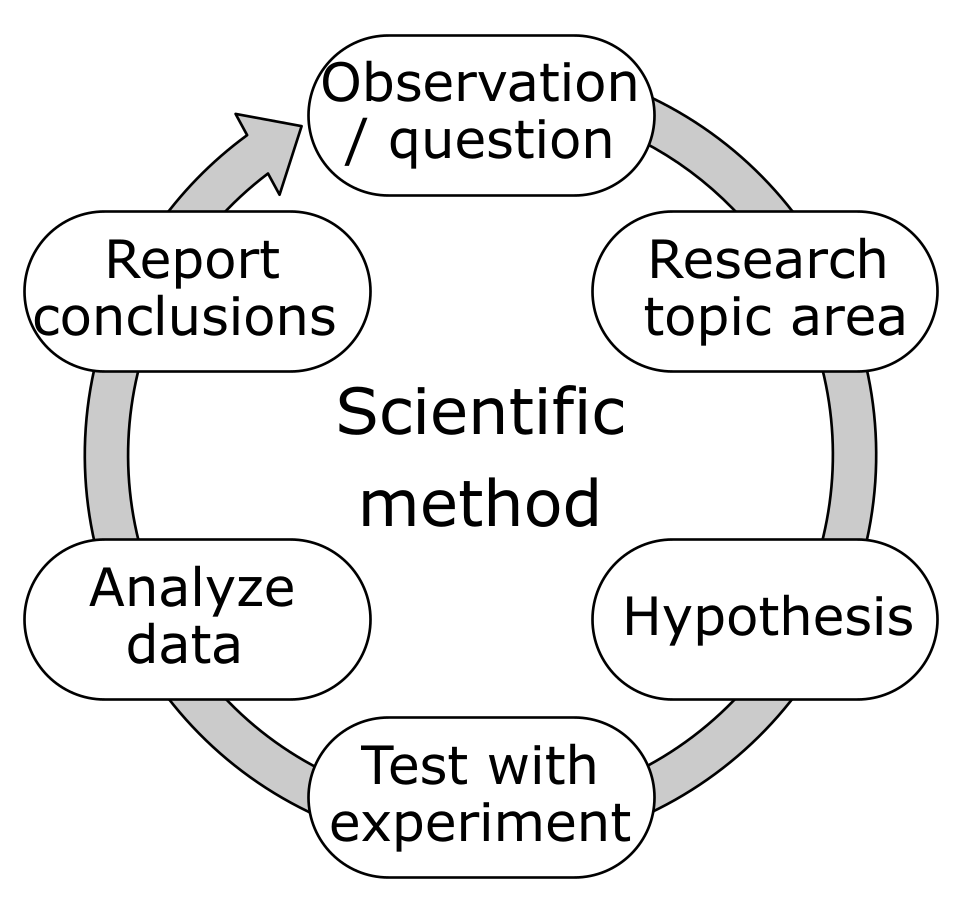
\includegraphics[width=\textwidth]{The_Scientific_Method.png}
\caption{Source: wikimedia.org, Author:  	Efbrazil}
\end{figure}
\end{column}
\end{columns}
\end{frame}

\section{Differential models}
\begin{frame}{Important differential equations in physics}
\begin{table}[H]
\centering
\begin{tabular}{rl}
Continuity & \(\pdv{\rho}{t} + \div\pab{\rho\vb{v}} = \sigma\) \\ [1em]
Diffusion & \(\pdv{\rho}{t} = \div\pab{\vb{D}\grad\rho}\) \\ [1em]
Harmonic oscillator & \(\odv[order=2]{\phi}{t} + \omega_{0}^{2}\phi = 0\) \\ [1em]
Euler-Lagrange & \(\odv{}{t}\pdv{\lagr}{\dot{q}_{i}} - \pdv{\lagr}{q_{i}} = 0\) \\ [1em]
Laplace & \(\laplacian V = 0\) \\ [1em]
Poisson & \(\laplacian V = -\frac{\rho}{\varepsilon_{0}}\) \\ [1em]
Helmholtz & \(\pab{\laplacian + k^{2}}V = 0\) \\ [1em]
Wave & \(\pab{\laplacian - \inv{c^{2}}\pdv[order=2]{}{t}}V = 0\)
\end{tabular}
\end{table}
\end{frame}

\end{document}